\begin{figure*}
    \begin{subfigure}[t]{0.16\linewidth}
        \centering
        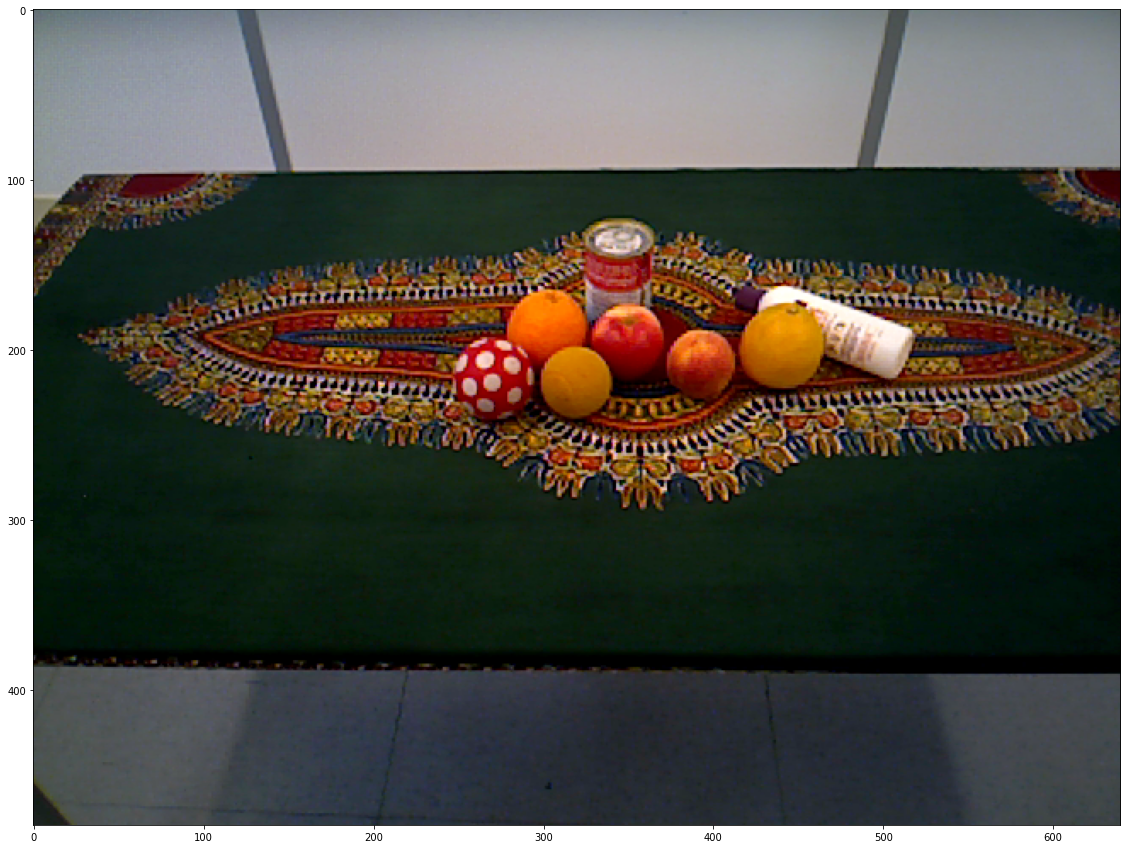
\includegraphics[width=\textwidth]{figures/methods1.png}
        \caption{Initial RGB}
        \label{methods:pic1}
    \end{subfigure}
    \hfill
    \begin{subfigure}[t]{0.16\linewidth}
        \centering
        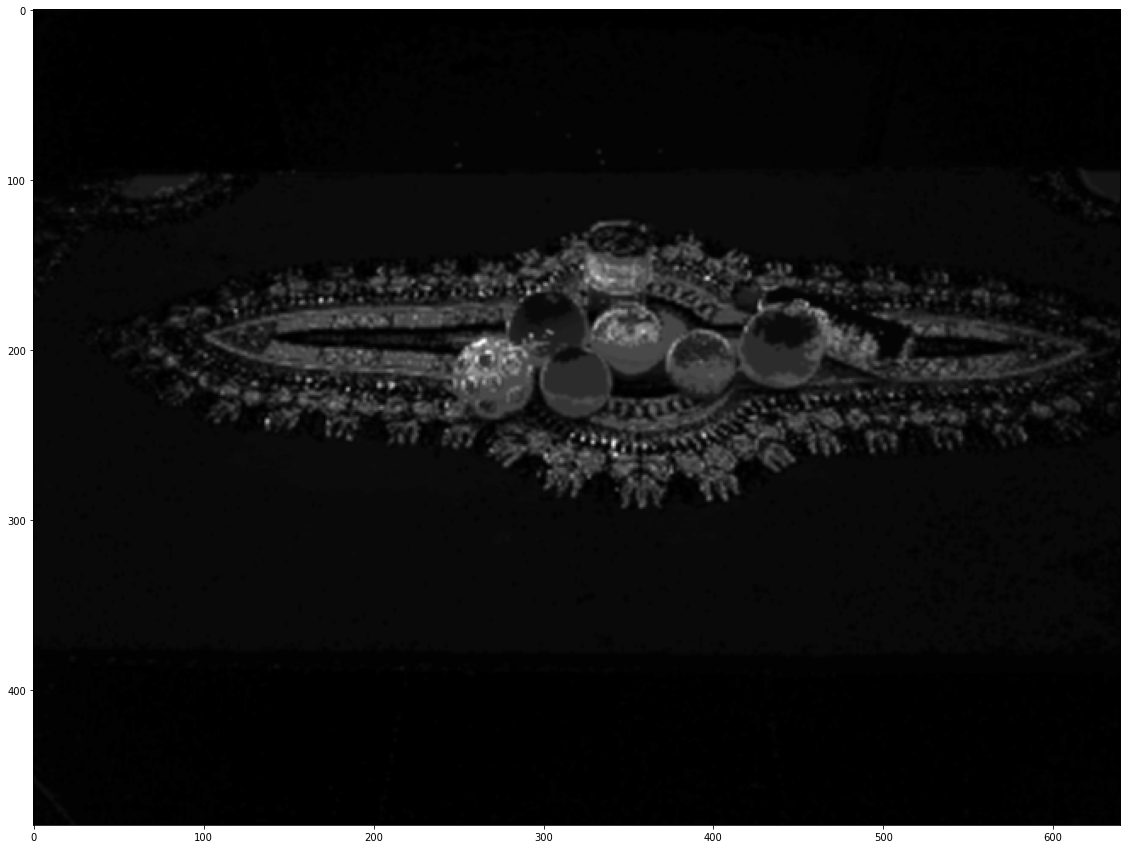
\includegraphics[width=\textwidth]{figures/methods2.png}
        \caption{Saliency map}
        \label{methods:pic2}
    \end{subfigure}
    \hfill
    \begin{subfigure}[t]{0.16\linewidth}
        \centering
        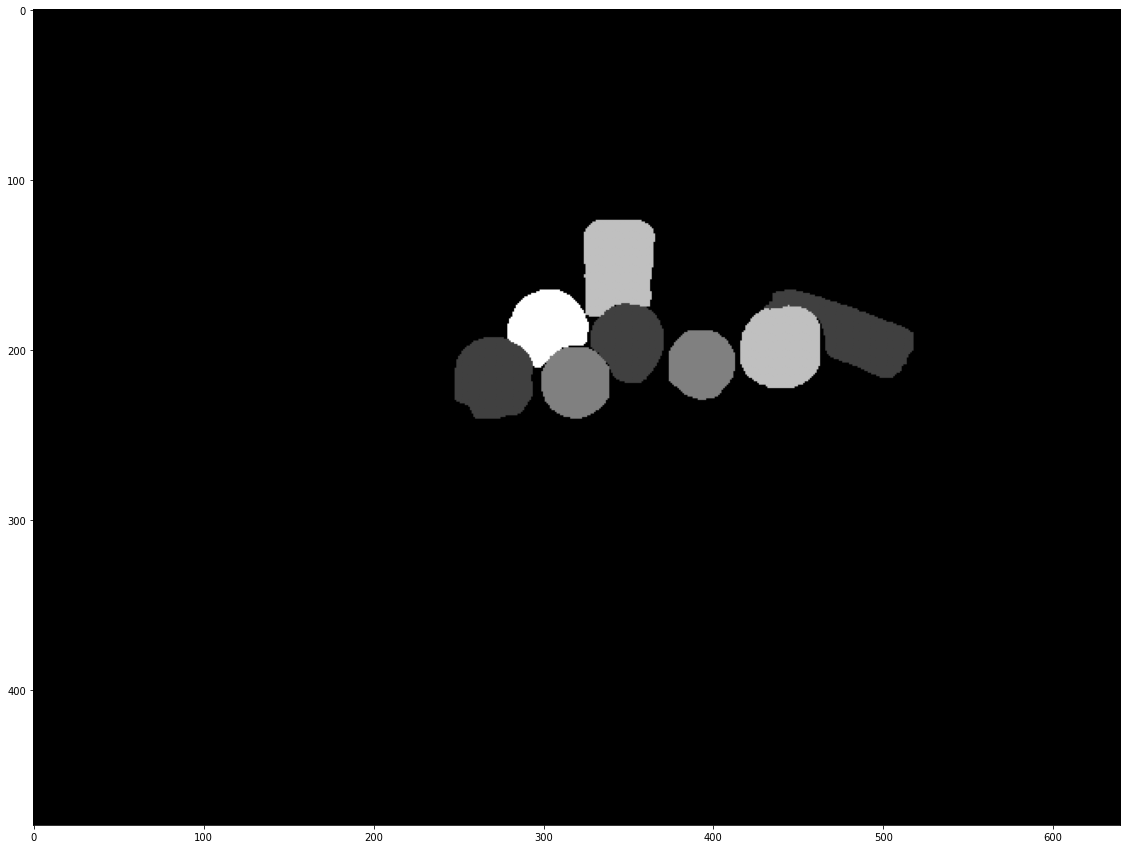
\includegraphics[width=\textwidth]{figures/methods3.png}
        \caption{Segmentation before recoloring}
        \label{methods:pic3}
    \end{subfigure}
    \hfill
    \begin{subfigure}[t]{0.16\linewidth}
        \centering
        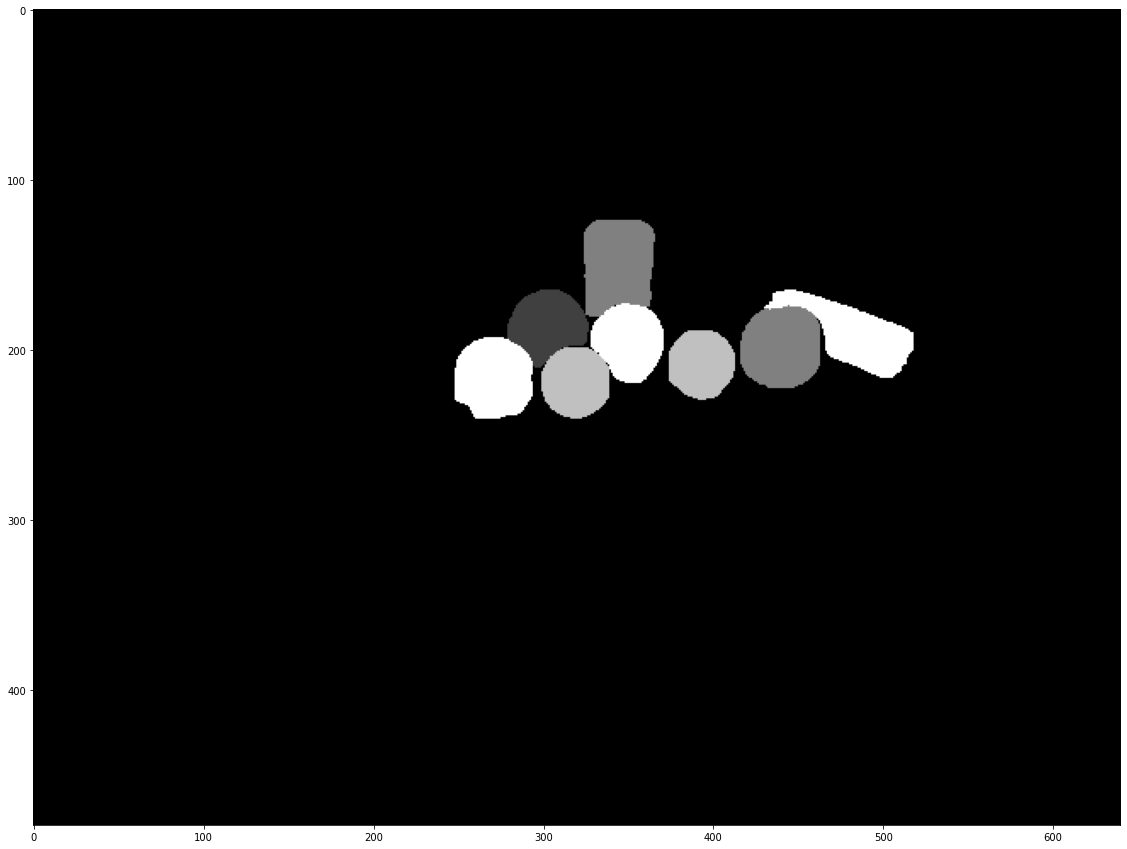
\includegraphics[width=\textwidth]{figures/methods4.png}
        \caption{Segmentation after recoloring}
        \label{methods:pic4}
    \end{subfigure}
    \hfill
    \begin{subfigure}[t]{0.16\linewidth}
        \centering
        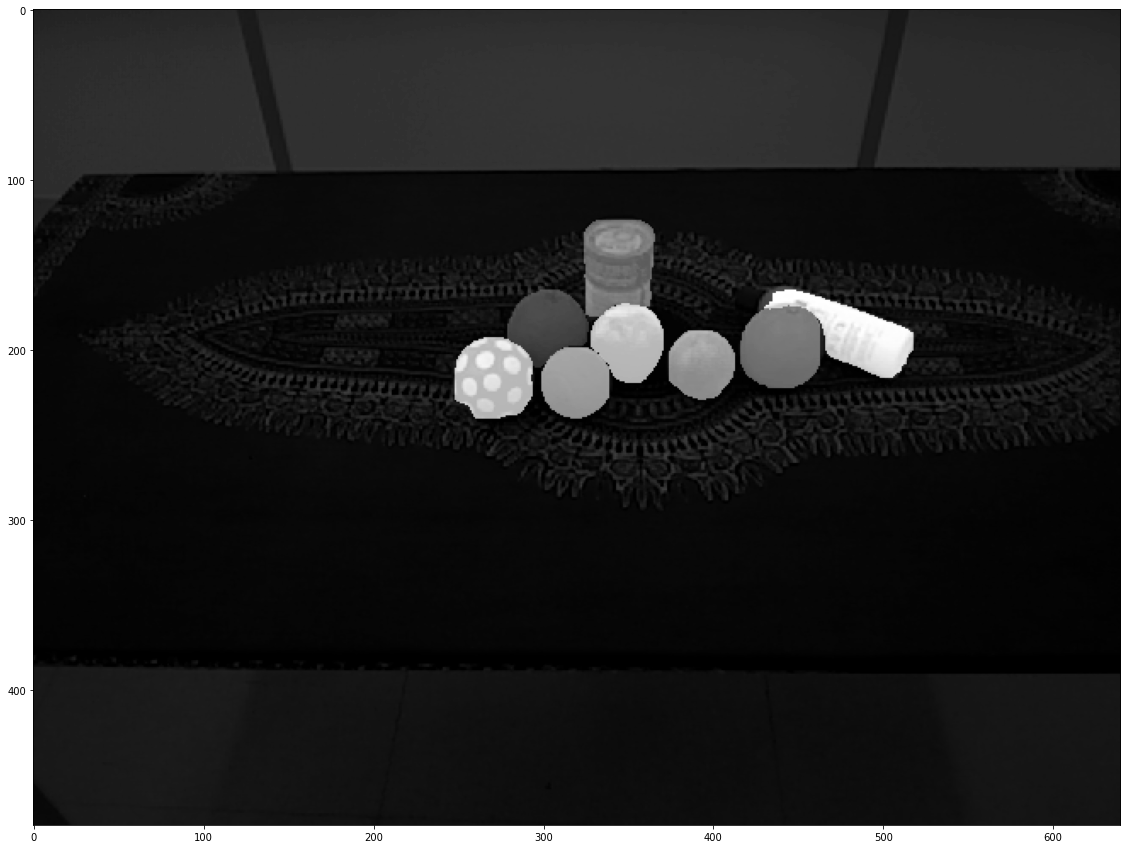
\includegraphics[width=\textwidth]{figures/methods5.png}
        \caption{Our result}
        \label{methods:pic5}
    \end{subfigure}
    \newline
    \begin{subfigure}[t]{0.16\linewidth}
        \centering
        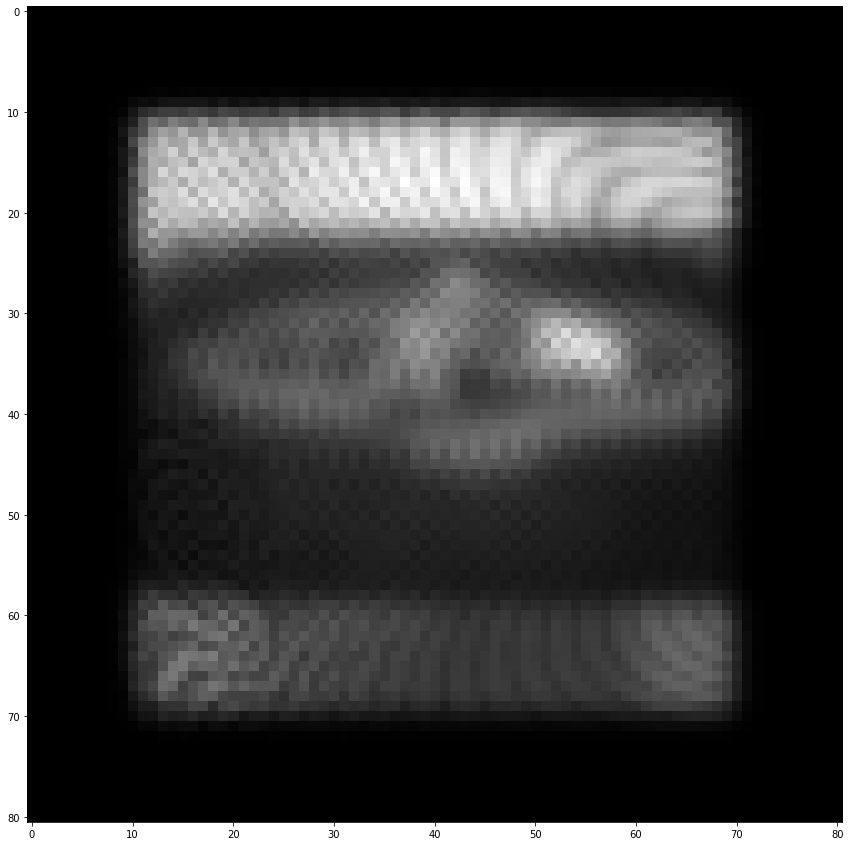
\includegraphics[width=\textwidth]{figures/methods6.png}
        \caption{p2p: initial RGB}
        \label{methods:pic6}
    \end{subfigure}
    \hfill
    \begin{subfigure}[t]{0.16\linewidth}
        \centering
        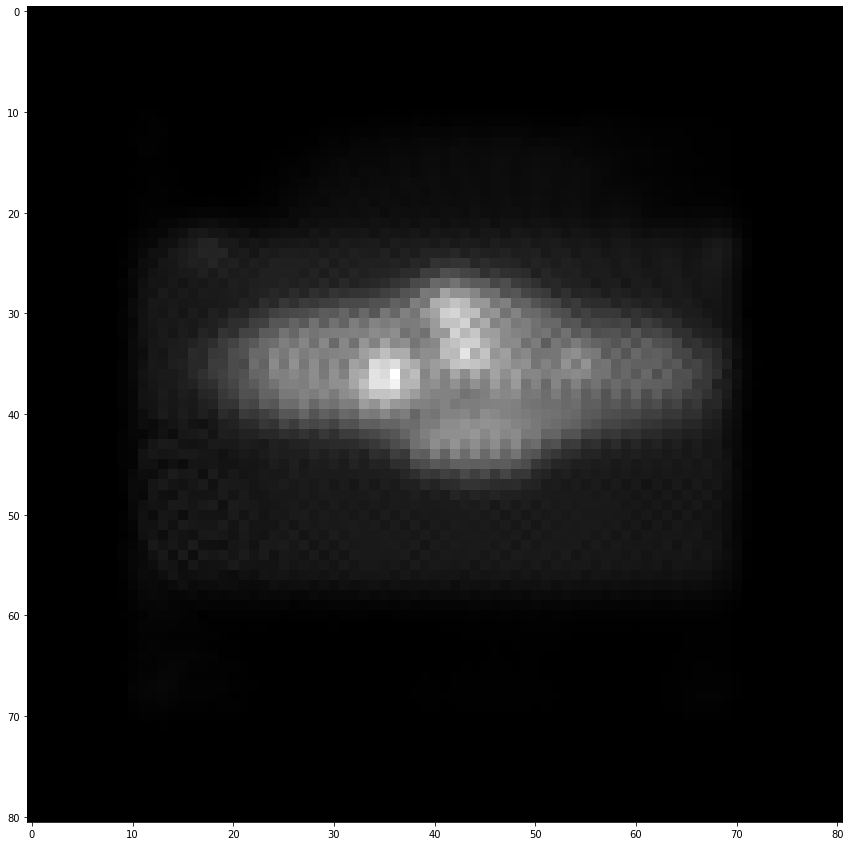
\includegraphics[width=\textwidth]{figures/methods7.png}
        \caption{p2p: saliency map}
        \label{methods:pic7}
    \end{subfigure}
    \hfill
    \begin{subfigure}[t]{0.16\linewidth}
        \centering
        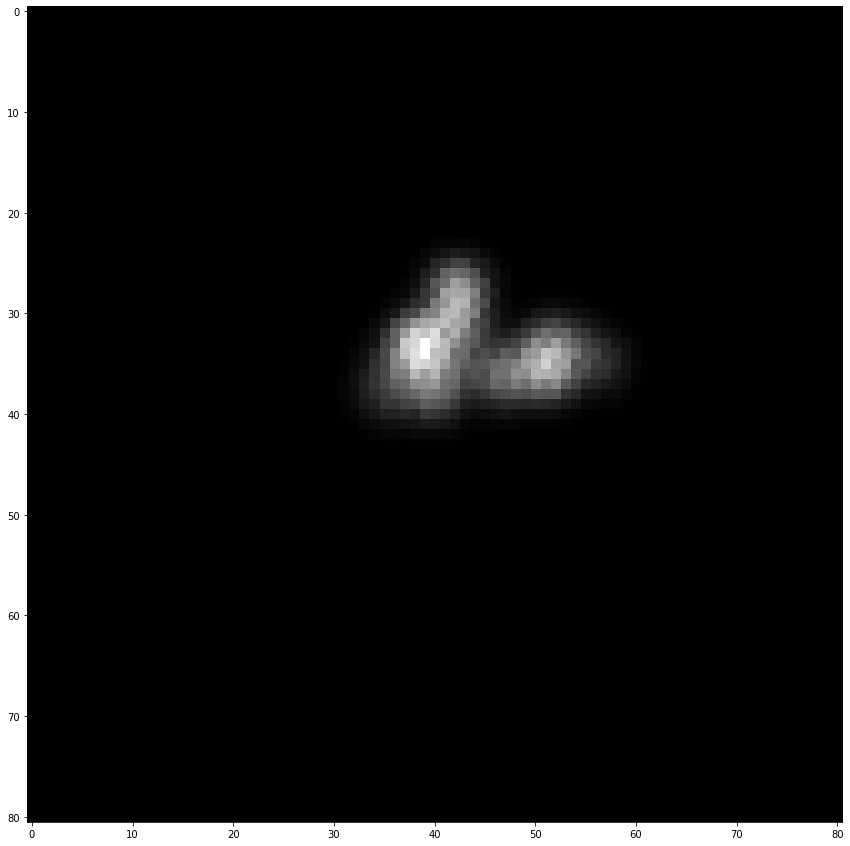
\includegraphics[width=\textwidth]{figures/methods8.png}
        \caption{p2p: segmentation before recoloring}
        \label{methods:pic8}
    \end{subfigure}
    \hfill
    \begin{subfigure}[t]{0.16\linewidth}
        \centering
        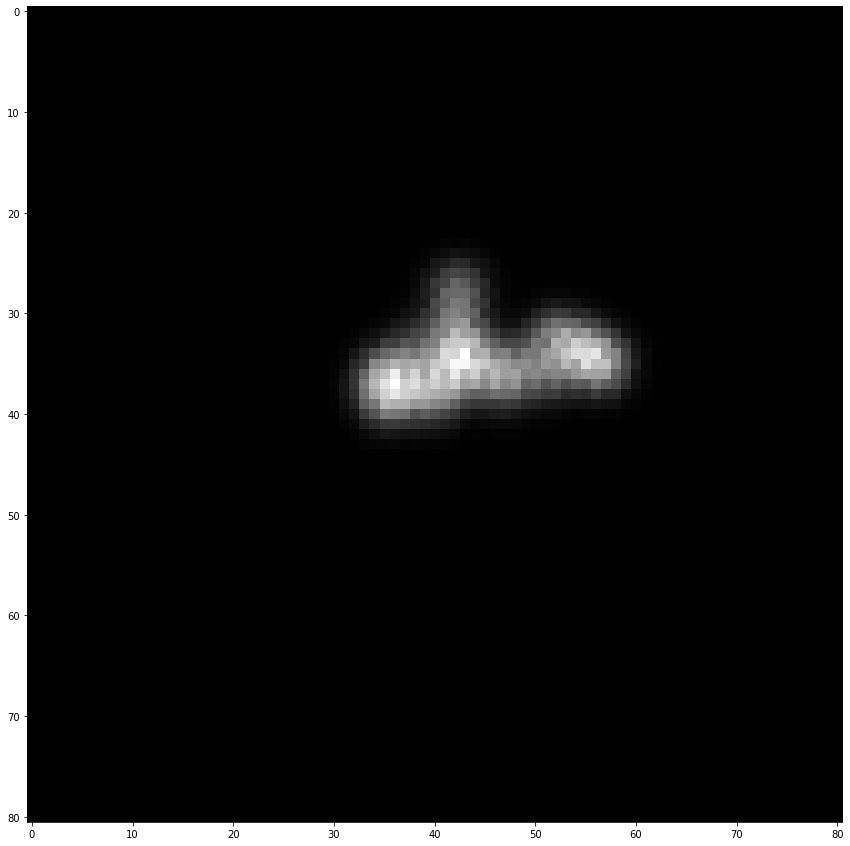
\includegraphics[width=\textwidth]{figures/methods9.png}
        \caption{p2p: segmentation after recoloring}
        \label{methods:pic9}
    \end{subfigure}
    \hfill
    \begin{subfigure}[t]{0.16\linewidth}
        \centering
        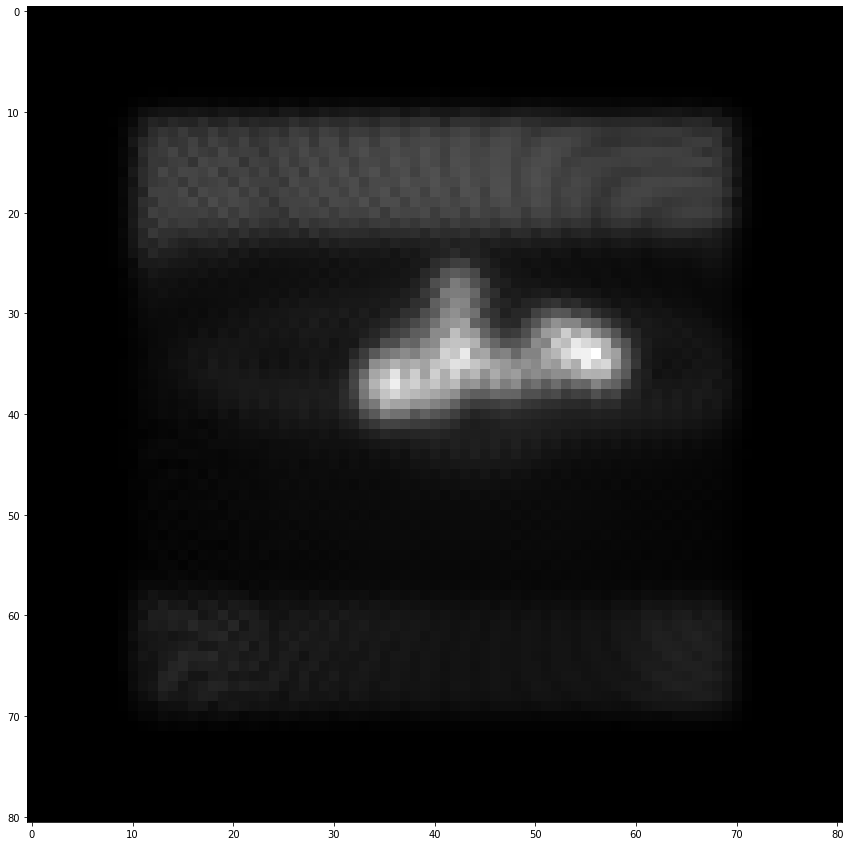
\includegraphics[width=\textwidth]{figures/methods10.png}
        \caption{p2p: our result}
        \label{methods:pic10}
    \end{subfigure}
    \caption{Stages of processing the picture and corresponding visualizations via pulse2percept.}
    \label{methods:picture}
    \Description{Initially, the image is converted to grayscale, then the saliency map and segmentation map are obtained. After that, all these maps and grayscale images are combined in the resulting image. Finally, visualization via pulse2percept is added to show improvements to bionic vision implant users.}
\end{figure*}
